\documentclass[a4paper,12pt]{article}

\usepackage[left=25mm, right=25mm, top=25mm, bottom=25mm]{geometry}

\usepackage{amsmath}
\usepackage{amssymb}
\usepackage{amsfonts}
\usepackage[style=iso]{datetime2}
\usepackage[explicit]{titlesec}
\usepackage{amsthm}
\usepackage{mathrsfs}
\usepackage{array}
\usepackage{graphicx}
\usepackage{mathtools} % Provides \mathrlap command
\usepackage{xparse}
\usepackage{float}
\usepackage[skip=1em,indent]{parskip}
\usepackage{caption}
\usepackage[colorlinks=true, linkcolor=black]{hyperref}
\usepackage{tocloft}
\usepackage{enumitem}
\usepackage[toc, page]{appendix}
\usepackage{accents}
\usepackage[perpage, symbol*]{footmisc} % for dagger footnotes
\DefineFNsymbols{sym}{\textdagger \textdaggerdbl \textsection \textparagraph %
{\textdagger\textdagger} {\textdaggerdbl\textdaggerdbl} %
{\textsection\textsection} {\textparagraph\textparagraph}}
\setfnsymbol{sym}

\usepackage{tikz}
\tikzset{>=latex} % for LaTeX arrow head
\usepackage{pgfplots} % for the axis environment
\usetikzlibrary{calc,decorations.markings}

\pgfplotsset{compat=1.18, every tick label/.append style={font=\footnotesize}}

\graphicspath{ {./Images/} }

\makeatletter
\def\th@plain{%
  \thm@notefont{}% same as heading font
  \itshape % body font
}
\def\th@definition{%
  \thm@notefont{}% same as heading font
  \normalfont % body font
}
\makeatother

\newcommand*\diff{\mathop{}\!d} % for the differential in integrals
% ---------------- %
\ExplSyntaxOn %* This command is for row vectors; unstarred version has no delimiter scaling for inline; starred version has delimiter scaling for display
\seq_new:N \l_user_rvec_seq

% expl3 worker (does the splitting/formatting)
\cs_new_protected:Npn \dbacc_rvec:n #1
 {
  \seq_clear:N \l_user_rvec_seq
  \seq_set_split:Nnn \l_user_rvec_seq { , } { #1 }
  \seq_use:Nn \l_user_rvec_seq { \enspace }
 }

% plain-name wrapper (no ':' in its name) — safe to call outside ExplSyntaxOn
\cs_new_protected:Npn \dbaccrvec #1 { \dbacc_rvec:n { #1 } }

% user-level \rvec interface (star + optional size + mandatory arg)
\NewDocumentCommand \rvec { s o m }
 {
  \IfBooleanTF{#1}
    { \left[\,\dbaccrvec{#3}\,\right] } % starred -> automatic \left...\right
    { \IfValueTF{#2}
        { \mathopen{#2[}\,\dbaccrvec{#3}\,\mathclose{#2]} } % sized optional arg
        { [\,\dbaccrvec{#3}\,] } % default small delimiters
    }
 }
\ExplSyntaxOff
% ---------------- %
\newcommand{\R}{\mathbb{R}}
\newcommand{\C}{\mathbb{C}}
\newcommand{\Z}{\mathbb{Z}}

\NewCommandCopy{\oldIm}{\Im}
\renewcommand{\Im}{\mathop{\oldIm\mathfrak{m}}}
\NewCommandCopy{\oldRe}{\Re}
\renewcommand{\Re}{\mathop{\oldRe\mathfrak{e}}}

\newcommand{\overbar}[1]{\mkern 1.5mu\overline{\mkern-1.5mu#1\mkern-1.5mu}\mkern 1.5mu}

\DeclareMathOperator{\Res}{Res}

\DeclarePairedDelimiterX{\norm}[1]{\lVert}{\rVert}{#1}
\DeclarePairedDelimiterX{\abs}[1]{\lvert}{\rvert}{#1}
% ---------------- %
\newcommand{\ihat}{\boldsymbol{\hat{\imath}}}
\newcommand{\jhat}{\boldsymbol{\hat{\jmath}}}
\newcommand{\khat}{\boldsymbol{\hat{k}}}
\newcommand{\ehat}{\mathbf{\hat{e}}}
\newcommand{\T}{\mathrm{T}}
% ---------------- %

\newtheorem{theorem}{Theorem}
\newtheorem{lemma}[theorem]{Lemma}
\newtheorem{proposition}[theorem]{Proposition}
\newtheorem{corollary}{Corollary}[theorem]

\theoremstyle{definition}
\newtheorem{definition}[theorem]{Definition}
\newtheorem{example}[theorem]{Example}

% \setlength{\cftsecnumwidth}{3em}

\begin{titlepage}
\title{Introduction to Differential Forms}
\author{Abdul Musthakin}
\date{October 2025}
\end{titlepage}

% \renewcommand{\thesection}{\Roman{section}}

\allowdisplaybreaks

\setlength{\parindent}{0pt}

\begin{document}
\maketitle

\tableofcontents

\pagebreak

\section*{Prerequisites}

\begin{itemize}
    \item Single-variable calculus
    \item Vectors
\end{itemize}

\section{Introduction \& Motivation}

Understanding what an integral means, in a general sense, is not particularly difficult.
Given a function, it is pretty easy to draw it as a curve on a graph.
By looking at its graph, and choosing some interval on the $x$-axis, we can see the area between the curve and the $x$-axis.
This (signed) area is what is calculated by an integral.
\begin{figure}[H]
\centering
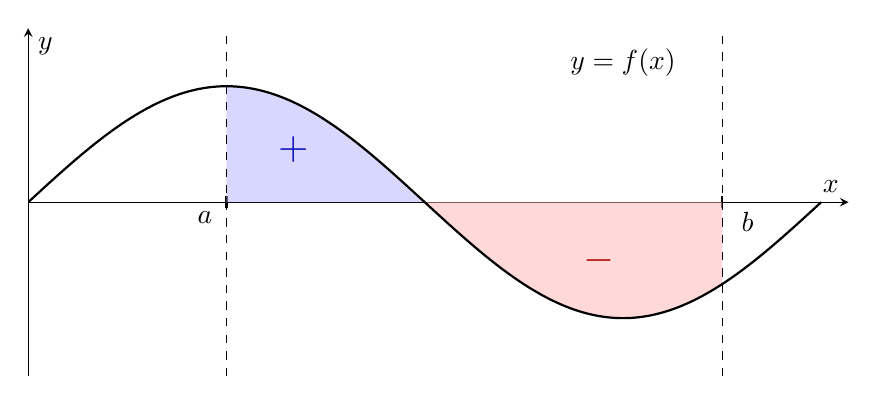
\begin{tikzpicture}
\begin{axis}[
    width=12cm,
    height=6cm,
    axis lines=middle,
    xlabel={$x$},
    ylabel={$y$},
    xmin=0, xmax=6.5,
    ymin=-1.5, ymax=1.5,
    xtick={1.5708, 5.49779},
    xticklabels={},
    ytick=\empty,
    samples=200,
    domain=0:2*pi,
    enlargelimits=false,
    tick style={black, thick},
    major tick length=0.15cm,
]

% Labels for a and b
\node[below] at (axis cs:1.4, 0) {$a$};
\node[below] at (axis cs:5.7, 0) {$b$};

% Shaded area for positive region (a to π)
\addplot[fill=blue!30, opacity=0.5, domain=1.5708:3.14159, draw=none] 
    {sin(deg(x))} \closedcycle;

% Shaded area for negative region (π to b)
\addplot[fill=red!30, opacity=0.5, domain=3.14159:5.49779, draw=none] 
    {sin(deg(x))} \closedcycle;

% The sin(x) function
\addplot[black, thick, domain=0:2*pi] {sin(deg(x))};

% Vertical lines at x=a and x=b
\addplot[dashed, black] coordinates {(1.5708, -1.5) (1.5708, 1.5)};
\addplot[dashed, black] coordinates {(5.49779, -1.5) (5.49779, 1.5)};

% Label for the function
\node[above, black] at (axis cs:4.71239, 1) {$y = f(x)$};

% Labels for areas
\node[blue!70!black, font=\Large] at (axis cs:2.1, 0.45) {$+$};
\node[red!70!black, font=\Large] at (axis cs:4.52, -0.5) {$-$};

\end{axis}
\end{tikzpicture}
\caption{A definite integral}
\label{fig:definite_integral_sin}
\end{figure}
The area illustrated by the above figure is given by
\begin{equation*}
    \int_{a}^{b} f(x) \diff x.
\end{equation*}
Now, everything that was just stated has many asterisks.
We can have functions that cannot be integrated, or at least, not in the `usual' sense.
Even if we can integrate a function, we might not be able to get our integral (and thus desired area) in terms of functions that we are used to.
Even if we ignore all of that, there is plenty of theory regarding how we define integrals -- extending and generalizing to different applications.
So it turns out that integrals are not that simple, but their idea is.

The above refers specifically to definite integrals, and so too will further discussion.
It would thus be useful to have a brief mention of indefinite integrals for the sake of completeness.
An indefinite integral of some function $f$ is itself not a number, nor even a function.
It is a class of functions,\footnote{An equivalence class.} whose shared property is that their derivative is $f$.
A member of this class is referred to as an antiderivative of $f$, and it can be written as
\begin{equation*}
    F(x) \coloneq c + \int_{a}^{x} f(t) \diff t,
\end{equation*}
where $a$ and $c$ are some constants.
Since any antiderivative (and thus the indefinite integral) of a function can be rewritten in terms of a definite integral, there is nothing regarding the former concept that warrants its mention in the discussions ahead.

Consider the notation we use for integrals.
We have a unique symbol, $\int$, to always know when we are integrating.
We have the integrand after that, which is what we are integrating.
Also, we have the start and end points of our interval which we are integrating over.
Finally, we have something on the end.
It is definitely not useless, as it tells us what variable we are integrating with respect to.
For instance, it is true that
\begin{equation*}
    \int_{a}^{b} f(x) \diff x = \int_{a}^{b} f(t) \diff t = \int_{a}^{b} f(u) \diff u,
\end{equation*}
just as it is true that
\begin{equation*}
    \sum_{i=1}^{n} f(i) = \sum_{j=1}^{n} f(j) = \sum_{k=1}^{n} f(k).
\end{equation*}
The exact symbol we use for the variable does not matter; they are just labels for the same thing.
Now, in the context of sums, you can simply expand out to show that they are the same thing.
They all refer to $f(1) + f(2) + f(3) + \ldots + f(n)$.
It is not so straightforward for integrals, but the idea holds.
We could leave it at that, and say that the differential is just a part of the notation that conveys some useful information.
There is much more to it than that, however.

The word `differential' has many meanings in mathematics, and it can refer to completely different concepts in different fields (or even in the same field).
One thing that it can refer to is an infinitesimal -- a number closer to zero than any real number that is not itself zero.
Leibniz was the first to coin the term for that usage, although the idea of infinitesimals date back to \href{https://plato.stanford.edu/entries/continuity/}{ancient Greek mathematicians}.

Early developments in calculus throughout the 17th and 18th centuries by the likes of Newton and Leibniz were noticeably reliant on the idea of infinitesimals.
That itself was not a bad thing, but that the lack of rigour was.
We would see the development of a more rigourous foundation of calculus by mathematicians in the 19th century, particularly Cauchy.
Infinitesimals would be left in favour of limits, and the latter is the formulation that is universally taught in schools.
\begin{figure}[H]
\centering
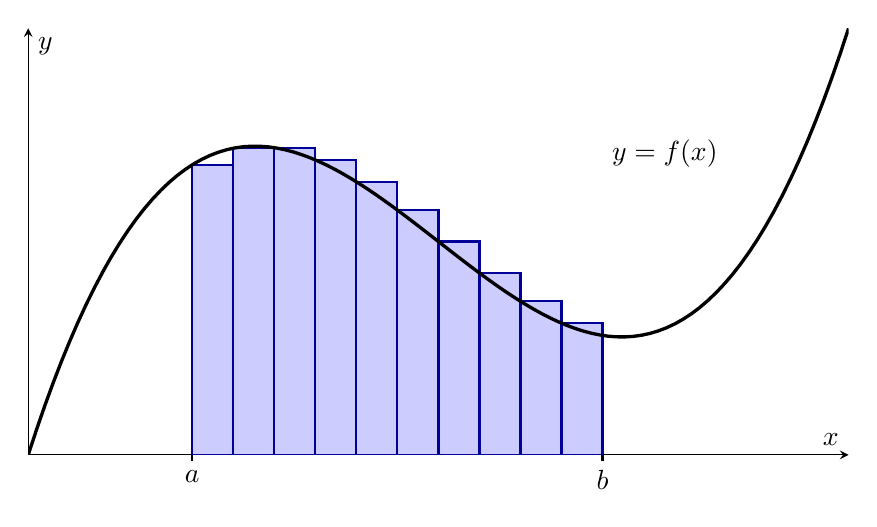
\begin{tikzpicture}
\begin{axis}[
    width=12cm,
    height=7cm,
    axis lines=middle,
    xlabel={$x$},
    ylabel={$y$},
    xmin=0, xmax=10,
    ymin=0, ymax=100,
    xtick={2, 7},
    xticklabels={$a$, $b$},
    ytick=\empty,
    samples=100,
    domain=0:10,
    enlargelimits=false,
    tick style={black, thick},
    major tick length=0.15cm,
    xticklabel style={font=\normalsize},
]


% Draw Riemann sum rectangles (left endpoint)
\foreach \i in {0,...,9} {
    \pgfmathsetmacro{\xleft}{2 + \i*0.5}
    \pgfmathsetmacro{\xright}{\xleft + 0.5}
    \pgfmathsetmacro{\height}{-15*(\xleft-5) + (\xleft-5)^3 + 50}
    \addplot[fill=blue!20, draw=blue!60!black, thick] coordinates {
        (\xleft, 0) (\xleft, \height) (\xright, \height) (\xright, 0)
    } -- cycle;
}

% The curve
\addplot[black, very thick, domain=0:10] {-15*(x-5) + (x-5)^3 + 50};

% Label for the function
\node[above right, black] at (axis cs:7, 65) {$y = f(x)$};

\end{axis}
\end{tikzpicture}
\caption{Riemann sum approximation of an integral}
\label{fig:riemann_sum}
\end{figure}
This information about differentials allows us to view the one attached to every integral in way beyond just useful notation.
Putting the formalism and rigourous defintions of integrals aside, they are fancy sums.
The area under a graph can be approximated by rectangles, as is shown by the above figure.
As the width of the rectangles decrease, the sums \href{https://commons.wikimedia.org/wiki/File:Riemann_sum_(leftbox).gif}{get closer} to the actual area under the curve.
That is, the limit of this sum is an integral.

Instead of thinking about it in terms of limits, we can imagine summing an infinite number of rectangles with infinitesimal width.
The height of a rectangle at some value of $x$ can be given by $f(x)$, so if the integral sums over areas, the $dx$ is the infinitesimal width.
This is all very impercise and non-technical language.
However, it is enough to give us an intuitive feel of what an integral is and what the differential that is always attached to it means.

There is more to the peculiar symbol, though, and integrals are probably not the first place one would have spotted them.
That would instead be with regard to derivatives.
Indeed, the notation $dy/dx$ -- also attributed to Leibniz -- is very commonly used to denote the derivative of $y$ with respect to $x$.
When it is first taught to students at school, the warning will be given that it does not represent a fraction.
It just looks like a fraction, and treating it like a fraction works out almost all the time.

The resemblence it has to a ratio between two quantities is no coincidence, as Leibniz intended it to be just that: a ratio of infinitesimals.
The symbols $dx$ and $dy$ were used to represent infinitely small changes in $x$ and $y$ respectively.
Whilst we have, for the most part, left these impercise notions behind, they will prove to be somewhat useful in understanding these symbols.\footnote{At the end of the day, the symbols mean whatever we want as long as it consistent with the rest of our maths. That is why I gave the easy way out at the beginning, saying that the differential symbol in the integral can just be considered a part of the notation. However, as is being demonstrated, we can go further.}

\section{Differential of a Function}

Firstly, consider the fact that the derivative has many different notations.
The derivative of a function $f$ at $x$ may be expressed as $f'(x)$.
It follows that
\begin{equation*}
    \frac{dy}{dx} = f'(x).
\end{equation*}
This is just equating two things that are defined to mean the exact same thing.
Now, although the left-hand side is not a fraction, what if we rewrote the equation as follows?
\begin{equation*}
    dy = f'(x) \diff x
\end{equation*}
The right-hand side now looks exactly like an integrand.
This looks promising, but we did say beforehand that $dy/dx$ is not a fraction.
So, are we allowed to do that?
No. The symbols $dx$ and $dy$ have not been given a meaning outside of when they appear in $dy/dx$, so it makes no sense to seperate them.
However, when something does not have meaning, we can always attempt to give it one and see where that leads us.

First, let $\Delta x$ be some real number, just as $x$ is.
Then, we can call $df$ the differential of $f$, a function of $x$.
The differential itself is a function of both $x$ and $\Delta x$, is defined as
\begin{equation*}
    df(x, \Delta x) \coloneq f'(x) \Delta x.
\end{equation*}
What was the point of that?
We went from performing an algebraic manipulation in a situation where it does not make sense, to creating a perfectly fine definition.
Since we have made it clear that $df$ is a function of two variables, we can write $df(x, \Delta x)$ as $df(x)$ or even $df$ (we are not changing the meaning).
The differential of the function $f(x) = x$ is given by
\begin{equation*}
    dx = 1 \cdot \Delta x = \Delta x
\end{equation*}
for all values of $x$.
This means that, even though $dx$ is technically still a function of $x$, we can just write $dx = \Delta x$.
With this, and by letting $y = f(x)$, we can rewrite our equation as
\begin{equation*}
    dy = f'(x) \diff x.
\end{equation*}
This looks exactly like what we already had, but now we have reached it by valid means.
We see that the differential $dy$ is defined in terms of $x$ and $dx$, and the differential $dx$ is essentially just some real number.
If we desired, we could go further to obtain $dy/dx = f'(x)$, but this can lead to confusion.
By that equation, $f'(x)$ equals a ratio of differentials that have each been seperately defined.
However, $f'(x)$ is can be expressed with Leibniz's notation as $dy/dx$ -- which is not a ratio.\footnote{We cannot redefine the derivative to be a ratio of our two differentials. Their definitions involve the derivative, so it would be circular. Instead, view it as evidence for the self-consistency of Leibniz's notation}
This is just something to note.

We have now obtained our third interpretation of the differential, a function of two real numbers $x$ and $\Delta x$.
This can be extended to higher-order differentials, as well as to the differentials of multivariable functions.
Its usefulness is in the fact that it represents the principal part of the change of a function.
To see what that exactly means, consider some function\footnote{Technically, $f$ is the function and $f(x)$ is the value of the function at $x$.} $y=f(x)$ between two points $x$ and $x + \Delta x$.
Let $x$ be fixed.
The change in $x$ values is $\Delta x$ and the change in $y$ values is $\Delta y \coloneq f(x + \Delta x) - f(x)$.

By the definition of the derivative, $\Delta y / \Delta x \to f'(x)$ as $\Delta x \to 0$.
This means that for small $\Delta x$, we have $\Delta y / \Delta x \approx f'(x)$.
If the difference (or error) is $\varepsilon$, then $\Delta y / \Delta x = f'(x) + \varepsilon$.
Rearranging gives us
\begin{align*}
    \Delta y &= (f'(x) + \varepsilon) \Delta x \\
    &= f'(x) \Delta x + \varepsilon \Delta x \\
    &= dy + \varepsilon \Delta x.
\end{align*}
The change in $y$ is equal to a linear function of $\Delta x$, $dy$, plus a (generally) nonlinear error term.
Thus, $dy$ is the linear (or principal) part of $\Delta y$.
As $\Delta x \to 0$, we require that $\varepsilon \Delta x / \Delta x = \varepsilon \to 0$, i.e. the error term shrinks to zero faster than $\Delta x$.
This means that $\Delta y \to d y$, and $\Delta y \approx dy$ for small $\Delta x$.

Let us look at one use case of this: approximating the values of functions.
What is the value of $\sqrt{90}$?
Since the function $y = \sqrt{x}$ is strictly increasing, we know that $\sqrt{90}$ will be between $\sqrt{81}=9$ and $\sqrt{100}=10$.
Let $x = 100$ and $\Delta x = -10$, so that $x + \Delta x = 90$.
Thus, $\Delta y = \sqrt{90} - \sqrt{100} = \sqrt{90} - 10$.
This means that $10 - \Delta y$ is the exact value of $\sqrt{90}$, but we do not know what $\Delta y$ is.
Our approximation from before comes in handy here.

The derivative of $\sqrt{x}$ is given by
\begin{equation*}
    f'(x) = \frac{1}{2\sqrt{x}}.
\end{equation*}
At $x=100$, we have $f'(x) = 1/20 = 0.05$.
This is all we need for our approximation.
\begin{align*}
    \sqrt{90} &= \Delta y + 10 \\
    &\approx dy + 10 \\
    &= f'(10) \Delta x + 10 \\
    &= 0.05 \cdot -10 + 10 \\
    &= 9.5
\end{align*}
The actual value of $\sqrt{90}$ is $9.47213595\ldots$, so we were just 0.62\% off.
The computations were incredibly easy, which is the case as long as we have nice values of the function and its derivative to work with.
We can illustrate the efficacy of this method with a diagram. 
\begin{figure}[H]
\centering
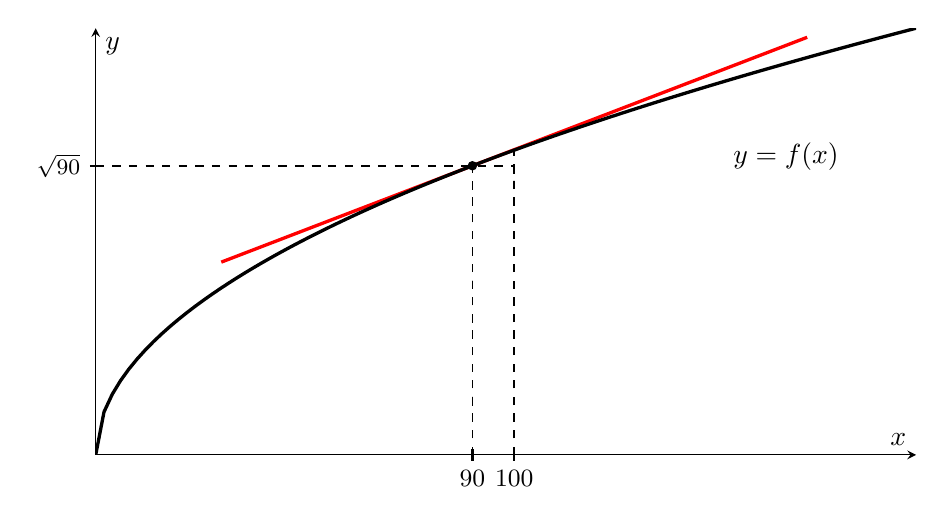
\begin{tikzpicture}
\begin{axis}[
    width=12cm,
    height=7cm,
    axis lines=middle,
    xlabel={$x$},
    ylabel={$y$},
    xmin=0, xmax=196,
    ymin=0, ymax=14,
    xtick={90, 100},
    xticklabels={90, 100},
    ytick={sqrt(90)},
    yticklabels={$\sqrt{90}$},
    samples=100,
    domain=0:196,
    enlargelimits=false,
    tick style={black, thick},
    major tick length=0.15cm,
    xticklabel style={font=\small},
]

\addplot[red, very thick, domain=30:170] {x/(2*sqrt(90)) + (sqrt(90) - 90/(2*sqrt(90)))};

% The curve
\addplot[black, very thick, domain=0:196] {sqrt(x)};

\draw[fill] (axis cs:{90,sqrt(90)}) circle [radius=1.5pt];
\addplot[black, semithick, dashed, domain=0:100] {sqrt(90)};
\addplot[black, semithick, dashed, domain=0:90] (90, {sqrt(x)});

\addplot[black, semithick, dashed, domain=0:100] (100, {sqrt(x)});

% Label for the function
\node[above right, black] at (axis cs:150, 9) {$y = f(x)$};

\end{axis}
\end{tikzpicture}
\caption{Linear approximation of $\sqrt{90}$}
\label{fig:linaer_approximation}
\end{figure}
We calculated $dy$, the increase in the tangent, as an approximation to $\Delta y$, the increase in the function.
As can be seen from the figure, these are very similar values.
Since $f'(x) \to 0$ as $x \to \infty$ (the curve flattens), this method of approximation gets better for larger square roots.
That does not mean that this method is not useful for other functions, as it is generally applicable to functions that are sufficiently `nice' -- where a discussion on `niceness' is besides the point.

Another example is approximating $\ln 3$.
We know that $\ln e$ is 1, and $e \approx 3$.
Let $x = e$ and $\Delta x = 3 - e$, so that $x + \Delta x = 3$.
Then, $\Delta y = \ln 3 - \ln e = \ln 3 - 1$.
The derivative of $\ln x$ is simply $1/x$, so we have
\begin{equation*}
    \ln 3 \approx \frac{1}{e} \cdot (3 - e) + 1 = \frac{3}{e}.
\end{equation*}
The number $e$ is well-known enough for us to use its value for the approximation, giving us $\ln 3 \approx 1.104$.
The actual value is $1.09861229\ldots$, which means that there is a 0.46\% error.
These approximations are known as linear approximations, and they have a fair bit of applications.
The idea of calculating the linear part of $\Delta y$ can be made more precise with \emph{Taylor's theorem}, though it is not necessary to understand the method itself.

\section{Reinterpreting Formulae}

Now that we have a formal definition of a differential, it would be useful to use what we have to look at commonly-known formulae in this new context.
First is the chain rule for derivatives.
Given two functions $f$ and $g$, the derivative of their composition $f \circ g$ is given by
\begin{equation*}
    f'(g(x)) g'(x).
\end{equation*}
If we write $y = f(g(x))$ and $u = g(x)$, then the previous fact can be rewritten as
\begin{equation*}
    \frac{dy}{dx} = \frac{dy}{du} \frac{du}{dx}
\end{equation*}
using Leibniz's notation.
The latter way is writing is more elegant both in this case, and for compositions of more than two functions.
It reinforces the idea of the derivative being a fraction, even though it is not.
If we were to, however, consider the terms on the RHS as being differentials, then we do have fractions -- which can cancel.
\begin{align*}
    \frac{dy}{du} \frac{du}{dx} = \frac{y'(x) \diff x}{u'(x) \diff x} \frac{u'(x) \diff x}{dx} = y'(x)
\end{align*}
Of course this is not a proof of the chain rule.
It does not show that the fraction $dy/du$ is the same as the derivative of $y$ with respect to $u$, and it does not work when $u'(x) = 0$ wherever we are differentiating at.
Regardless, it shows the chain rule to be intuitively very simple -- just `cancelling' fractions.

Our definition of differentials can also be shown to be insightful with regard to integration by substitution and the method of solving differential equations by seperation of variables.
That would make sense, as they are both linked to the chain rule (with the former being an inverse to some degree).
Given two functions $f$ and $g$, the integration by substitution formula states that
\begin{equation*}
    \int_{a}^{b} f(g(x))g'(x) \diff x = \int_{g(a)}^{g(b)} f(u) \diff u.
\end{equation*}
By making the substitution $u = g(x)$, we know that the differential of $u$ is given by $du = g'(x) \diff x$.
This suggests that the formula above is a literal substitution of one variable with another.
The limits being transferred from $x=a$ and $x=b$ to $u=g(a)$ and $u=g(b)$ make sense as well.\footnote{We could have had the limits on the RHS integral be $x=a$ and $x=b$ if we really wanted. This shows that nothing `actually' changes between the two integrals.}
Without the integral symbols, the equation would just be something that follows directly from the defintion of a differential.
If it were possible to integrate a differential in the sense of it being the whole integrand -- not just integrating a function -- then the formula would be completely trivial.

Now, on to the topic of differential equations.
Let $f$, $g$, and $h$ be functions that satisfy the differential equation
\begin{equation*}
    \frac{dy}{dx} = g(x)h(y),
\end{equation*}
with $y=f(x)$.
If we treat the $dy$ in $dy/dx$ as a differential (which is a bit awkward notationally but valid), then we have a fraction that can be seperated.
Multiplying both sides by $dx$ and dividing by $h(y))$ gives
\begin{equation*}
    \frac{dy}{h(y)} = g(x) \diff x.
\end{equation*}
This is really the same as
\begin{equation*}
    \frac{f'(x)}{h(f(x))} \diff x = g(x) \diff x.
\end{equation*}
Since $dx$ is some real number, we can cancel it out and then integrate both sides with respect to $x$ in order to solve the equation.
However, our integrals will have $dx$ at the end anyway.
What was the point of cancelling them out beforehand?
The $dx$ in an integral is still different from the $dx$ we have defined to be equal to some real number $\Delta x$.
Once again, if we could just integrate the differentials directly, things would be much simpler.

\section{Generalizing Differentials}

As was suggested at the end of the previous section, there is a different way to handle differentials that works well with integration.
Before that, we will have to perform quite a bit of work to generalize the notion of a differential; our current definition only works for functions of the type $\R \to \R$.
We will first cover higher-order differentials, which correspond to higher-order derivatives.
This is technically not a `generalisation' in that it requires no new definitions.
The second-order differenital, or second differential, of a function is given by finding the differential of the differential.
\begin{equation*}
    d^2 y \coloneq d(dy) = d(f'(x)\diff x) = (df'(x)) \diff x = f''(x) (dx)^2
\end{equation*}
Dividing through by $(dx)^2$ gives an equation very similar to Leibniz's notation for higher-order derivatives.
However, note that it is not a definition (as it would be if we were considering it as just notation).
\begin{equation*}
    \frac{d^2 y}{(dx)^2} = f''(x)
\end{equation*}
This is an interesting detail, again showing the efficacy and practicality of the notation.
Repeated applications of the differential gives us the general formula for the $n$-th order differential of $f$.
\begin{equation*}
    d^n y = d^n f(x, dx) = f^{(n)}(x) (dx)^n,
\end{equation*}
where $f^{(n)}$ is the $n$-th derivative of $f$.
This is pretty simple, but it only works under the assumption that $dx$ is itself not a function of $x$.
This might not be the case.
An example where $dx$ depends on $x$ is if $x$ depends on some parameter $t$.
The first-order differential is still given by $df(x, \Delta x) = f'(x) \Delta x = f'(x)\diff x$.
Since $x$ depends on $t$, $\Delta x$ depends on $t$ as well.\footnote{This is not a logical consequence, but rather a sensible choice we make. We choose to define $\Delta x$ as an actual change $x(t+\Delta t) - x(t)$, now that we are able to, instead of it just being some real number which represents the concept of change only when put in context.}
The principal part of the change $\Delta x$ is given by $dx = x'(t) \diff t$.
The reasoning for this is not new, as we are simply applying our definition of the differential to $x$ now that it is a function of $t$.
Then, $df$ is given by
\begin{equation*}
    df = f'(x)x'(t) \diff t.
\end{equation*}
This is essentially just the chain rule applied to differentials.
Finding $d^2 f$ will involve differentiating with respect to $t$ instead of $x$ to avoid concerning ourselves with whether $dx$ can be expressed as a function of $x$.
For this, we need the product rule.
\begin{equation*}
    d^2 f = f''(x) (x'(t)\diff t)^2 + f'(x) x''(t) (dt)^2
\end{equation*}
Simplifying this using $dx = x'(t)\diff t$ and $d^2 x = x''(t) (dt)^2$ gives us
\begin{equation*}
    d^2 f = f''(x) (dx)^2 + f'(x) d^2 x.
\end{equation*}
Note that differentiating with respect to $x$ directly would still have given us the same answer (even if it might not be technically valid).
This result generalizes to third derivatives, fourth derivatives, and so on.
The general formula for the $n$-th order differential is not at all insightful, so it will not be provided.
Higher-order differentials in general are not particularly relevant to the rest of our discussion, but they have been included for completeness.

Now we will consider multivariable functions.
Let $f\colon \R^n \to \R$, so it maps $n$ real numbers to a single real number.
It can equivalently be considered a function of $n$ independent variables, and we may write $y = f(x_1, \ldots, x_n)$.
There are multiple sensible ways of defining the differential.
We will first cover the simpler of the two approaches, before we cover the second and show that they are actually the same thing.
The total change in $y$ is given by
\begin{equation*}
    \Delta y = \Delta f \coloneq f(x_1 + \Delta x_1, \ldots, x_n + \Delta x_n) - f(x_1, \ldots, x_n),
\end{equation*}
where $\Delta x_i$ is a real number.
We are able to split this change into a linear (principal) part and a nonlinear part (which we call the error).
Each $x_i$ will contribute to the total change, both in its principal part and error part.
The former is given by
\begin{equation*}
    \frac{\partial y}{\partial x_i} \Delta x_i,
\end{equation*}
which we will calse the partial differential of $y$ with respect to $x_i$.
The error is simply $\varepsilon_i \Delta x_i$.
This is a natural extension of the one-dimensional case, with the primary difference being that we have now many more terms.
We can find the total principal change in $y$ due to the changes in all the variables by summing the partial differentials.
The result of this sum will be called the total differential of $y$.
\begin{equation*}
    dy \coloneq \sum_{i=1}^{n} \frac{\partial y}{\partial x_i} \Delta x_i
\end{equation*}
Since $dx_i(\Delta x_1, \ldots, \Delta x_n) = \Delta x_i$ (the partial derivative equals one for this term and zero for all others), we can rewrite the differential as
\begin{equation*}
    dy = \sum_{i=1}^{n} \frac{\partial y}{\partial x_i} \diff x_i.
\end{equation*}
As all $\Delta x_i \to 0$, we have $\varepsilon_i \to 0$, so $dy \to \Delta y$.
Just as in the case of one variable, this is approximately equal to the actual change in $y$: $\Delta y \approx \diff y$ (for small changes in $x_i$).
Their use cases are also similar.
However, their increased generality makes them much more applicable to situations -- including estimating error in measurements.

Since our function $f$ takes a list of numbers, and a list of numbers can be represented by a vector, we can consider $f$ to map $m$-dimensional vectors to real numbers.
This will not change anything about the above formula; we are now just considering the components of $\mathbf{x}$ and $d\mathbf{x}$.
We can go a step further by consider functions that output vectors as well.
Let $\mathbf{f}\colon \R^m \to \R^n$.
The only thing that changes is that we are now differentiating vectors, which we do by differentiating their components seperately.
This gives us a slightly modified formula for the total differential.
It is just a change of notation.
\begin{equation*}
    d\mathbf{f} = \sum_{i=1}^{n} \frac{\partial\mathbf{f}}{\partial x_i} \diff x_i
\end{equation*}
When we generalize to vector-valued functions, the changes in our function are no longer a real number.
It thus makes sense that the differential is not a real number anymore, either.
Functions that map vectors to vectors will be as general as we go for now.
Although, as we stated before, we will offer a different perspective on what we just derived.
Once again, consider $\mathbf{f}\colon \R^m \to \R^n$, with $\mathbf{x}$ and $\Delta\mathbf{x}$ being in $\R^m$.
The total change in $\mathbf{f}$ is given by
\begin{equation*}
    \Delta \mathbf{f} = \mathbf{f}(\mathbf{x} + \Delta\mathbf{x}) - \mathbf{f}(\mathbf{x}).
\end{equation*}
This is a rewritten version of what we had before.
We want this total change to be equal to a linear change, as well as an error term.
Note that we had $\Delta f = df + \varepsilon\Delta x$ in the one-dimensional case, with $df = f'(x) \diff x$.
Our multivariable version of the derivative is the Jacobian matrix, $\mathbf{J_f}$.
The linear change is then $\mathbf{J_f}\Delta\mathbf{x}$.
The error term is given by\footnote{It is not $\norm{\boldsymbol{\varepsilon}}\Delta\mathbf{x}$ instead because that would give an $n$-dimensional vector whilst the other terms are $m$-dimensional.} $\norm{\Delta\mathbf{x}}\boldsymbol{\varepsilon}$, with $\boldsymbol{\varepsilon} \to \mathbf{0}$ as $\Delta\mathbf{x} \to \mathbf{0}$.
We thus know that the total change in $\mathbf{f}$ can be expressed as follows.
\begin{equation*}
    \Delta\mathbf{f} = \mathbf{J_f}\Delta\mathbf{x} + \norm{\Delta\mathbf{x}}\boldsymbol{\varepsilon}
\end{equation*}
The differential of $\mathbf{f}$ is given by
\begin{equation*}
    d\mathbf{f}(\mathbf{x}, \Delta\mathbf{x}) = \mathbf{J_f}\Delta\mathbf{x}.
\end{equation*}
For $\mathbf{f}(\mathbf{x}) = \mathbf{x}$, it can be shown that the Jacobian $\mathbf{J_f} = \mathbf{I}$, the identity matrix.
This means that $d\mathbf{x} = \mathbf{I}\Delta\mathbf{x} = \Delta\mathbf{x}$ for all $\mathbf{x}$.
We can therefore rewrite the differential of $\mathbf{f}$ as
\begin{equation*}
    d\mathbf{f} = \mathbf{J_f} \diff\mathbf{x}.
\end{equation*}
This differential is exactly the same as the total differential we previously derived.
To show this, we simply perform the matrix multiplication.
\begin{equation*}
    \mathbf{J_f} \diff\mathbf{x} = \begin{bmatrix}
        \dfrac{\partial f_1}{\partial x_1} & \cdots & \dfrac{\partial f_1}{\partial x_n} \\[0.5em]
        \vdots & \ddots & \vdots \\[0.5em]
        \dfrac{\partial f_m}{\partial x_1} & \cdots & \dfrac{\partial f_m}{\partial x_n}
    \end{bmatrix}
    \begin{bmatrix}
        dx_1 \vphantom{\dfrac{\partial f_1}{\partial x_n}}\\[0.5em]
        \vdots \\[0.5em]
        dx_n \vphantom{\dfrac{\partial f_m}{\partial x_n}}
    \end{bmatrix}
    = \begin{bmatrix}
        \dfrac{\partial f_1}{\partial x_1}\diff x_1 + \cdots + \dfrac{\partial f_1}{\partial x_n}\diff x_n\\[0.5em]
        \vdots \\[0.5em]
        \dfrac{\partial f_m}{\partial x_1}\diff x_1 + \cdots + \dfrac{\partial f_m}{\partial x_n}\diff x_n
    \end{bmatrix}
    = \sum_{i=1}^{n} \frac{\partial\mathbf{f}}{\partial x_i} \diff x_i
\end{equation*}
Whilst the two results are equivalent, the form involving the Jacobian is usually preferred.
It is much more compact and clear (as long as the definition and notation is understood).
The Jacobian better represents the nature of a derivative of as a linear map and not necessarily a number.
As a bonus, $d\mathbf{f} = \mathbf{J_f} \diff\mathbf{x}$ maintains a similar form to the one-dimensional version of the differential.
The other form may be better-suited for quick computations, however.

We have now obtained an interpretation of the differential for a more general class of functions. 
It is a function of $\mathbf{x}$ and $d\mathbf{x}$, representing the principal change in the function.
This generalisation, and the work done to formalise the derivative of functions of type $\R^m \to \R^n$ falls under the concept of the \href{https://en.wikipedia.org/wiki/Fr%C3%A9chet_derivative}{Fre\'chet derivative}.
This derivative can be defined on even more general spaces, but that is beyond the scope of our discussion.

A useful concept that is related to -- but distinct from -- our definition of the differential is 

\section{Tangent Spaces}

WIP

\section{Differential Forms}

WIP %TODO MOTIVATE TANGENT SPACES
%TODO GO THROUGH MATRICES SECTION AND ADD A BIT ON IDENTITY MATRIX AND DETERMINENTS AND INVERSES

\begin{appendices}

\section{Vectors \& Matrices} \label{appendix:vectors_and_matrices}

\subsection{Definition of a Vector} \label{appendix:vector_def}

An introduction to the concept of vectors usually involve giving examples of vectors -- such as arrows in a plane -- without giving a proper definition of what a vector is in general.
That makes sense, since such a definition is (relatively) technical and unecessary for simply working with vectors.
The technical definition is that a vector is an element of a vector space, but that alone simply replaces one question with another.
It follows that a definition of a vector space is now required.

To come up with it, we will follow a method of generalisation that can be readily applied to other situations as well.
We know that ordered pairs of real numbers are examples of vectors, so the set containing all such pairs is an example of a vector space.\footnote{This is technically an abuse of language. A vector space is a set with additional structure -- the ability to add and scale its elements in a certain way. However, this distinction is not very useful until we actually define a vector space properly.}
This set is denoted by $\R \times \R$, and $\R^2$ is a useful shorthand.
We will examine the properties of this set in order to obtain a general definition of a vector space.

Two things we can do with our vectors is add them together and scale them.
For the example we are working with, this is done component-wise: $(a, b) + (b, c) = (a + b, c + d)$ and $c \cdot (a, b) = (ac, bc)$.
Since we can use real numbers to scale vectors, they are also referred to as scalars in this context.
Both of those functions have geometric interpretations if the vectors are viewed as arrows on a plane.
Vector addition involves connecting two vectors tip-to-tail and the sum is the third side of a triangle (or the diagonal of a parallelogram).
Scalar multiplication involved literally scaling the length of a vector by some number, where multiplication by a negative number reverses direction.

Whilst vectors in general are not arrows, the way they add and scale is fundamental to them.
If we try to extract all the properties of addition and scalar multiplication, we get the following list.
Note that the boldface letters are elements of $\R^2$, whilst the greek letters are real numbers.
Also, the boldface zero represents (0, 0).
\begin{enumerate}
\item $\mathbf{u} + \mathbf{v} = \mathbf{v} + \mathbf{u}$
\item $\mathbf{u} + (\mathbf{v} + \mathbf{w}) = (\mathbf{u} + \mathbf{v}) + \mathbf{w}$
\item $\mathbf{0} + \mathbf{v} = \mathbf{v}$
\item $-\mathbf{v} + \mathbf{v} = \mathbf{0}$
\item $\lambda(\mu\mathbf{v}) = (\lambda\mu)\mathbf{v}$
\item $1\mathbf{v} = \mathbf{v}$
\item $\lambda(\mathbf{v} + \mathbf{w}) = \lambda\mathbf{v} + \lambda\mathbf{w}$
\item $(\lambda + \mu)\mathbf{v} = \lambda\mathbf{v} + \mu\mathbf{v}$
\end{enumerate}
That leads to our definition of a vector space -- a set, together with vector addition and scalar multiplication, that satisfies the above statements.\footnote{Addition and scalar multiplication must be closed, but this is within their definitions, rather than being a part of the axioms.}
More precisely, the third and fourth statements say that an identity vector (that works for all vectors) and inverse vectors (that each work for a specific vector) exist.
These statements are known as the vector space axioms.
Note that choosing those specific axioms to define a vector space is just that: a choice.\footnote{It is not an arbitrary choice, however. Vectors are an incredibly useful concept both in pure maths and in other subjects -- where they are applied (along with linear algebra in general) perhaps more than any other topic in maths.}
We can explore sets with different strucutres, obtains objects like groups and rings instead.

\subsubsection*{Basis and Dimension}

Two fundamental properties of vector spaces are their basis and dimension.
A \emph{basis} of a vector space $V$ is a set of vectors in $V$ that satisfies two key properties: the vectors are linearly independent, and they span the entire space.
Linear independence means that no vector in the set can be written as a linear combination of the others.
Spanning means that every vector in $V$ can be expressed as a linear combination of the basis vectors.

For example, in $\R^2$, the standard basis consists of $\ihat = (1, 0)$ and $\jhat = (0, 1)$.
Any vector $(a, b)$ in $\R^2$ can be written as $a\ihat + b\jhat$, showing that these vectors span $\R^2$.
They are also linearly independent, since neither can be written as a scalar multiple of the other.
Another basis for $\R^2$ could be $\{(1, 1), (1, -1)\}$, demonstrating that bases are not unique.

The \emph{dimension} of a vector space is the number of vectors in any basis for that space.
A remarkable theorem in linear algebra states that all bases of a given vector space have the same number of elements, making dimension well-defined.
For $\R^n$, the dimension is $n$, as the standard basis $\{\ehat_1, \ehat_2, \ldots, \ehat_n\}$ contains $n$ vectors, where $\ehat_i$ has a 1 in the $i$-th position and 0 elsewhere.
The dimension provides a measure of the ``size'' or ``degrees of freedom'' of the vector space.

A common notation for vectors is boldface letters, and that is what will be used in this document.
Regular real numbers are never in boldface, though they might use either the Latin or Greek alphabet.
Additionally, whilst there are many different objects that classify as vectors, the only ones that will be considered by us are in fact lists of real numbers.
An ordered listed of $n$ real numbers is an element of $\R^n$.
In this context, $n$ is always interpreted as being a positive integer.

The above contains sufficient information to define vectors and work with them on a basic level.
What follows are some additional points of discussion.
Firstly, there are many different notations that exist for vectors.
Arrows, particularly in physics, can also be used to denote vectors, e.g. $\vec{F} = m\vec{a}$.
It is not easy to write boldface symbols in handwriting, so another alternative is underlining the vector, $\underline{v}$, or putting a tilde beneath it, $\underaccent{\sim}{v}$.
For the actual value of the vector, you can write it as a coordinate, as was shown before.
Another common way is to write it as a column of numbers.
\begin{equation*}
    \mathbf{v} = \begin{bmatrix}
        a \\
        b
    \end{bmatrix}
\end{equation*}
It can be written also be written like as $\mathbf{v} = \rvec{a,b}$. Note that the former is called a column vector, whilst the latter is a row vector.
Technically, they are different objects, but this distinction only matters when dealing with matrices.
Another way to write a vector is $\mathbf{v} = \langle a, b \rangle$.
This might be preferred due to avoiding confusion with coordinates.
Additionally, given that $\ihat = \langle 1, 0 \rangle$ and $\jhat = \langle 0, 1 \rangle$, you can write a vector as $\mathbf{v} = v_x\ihat + v_y\jhat$, where $v_x$ and $v_y$ are the components of the vector.
Note that these examples were given for $\R^2$, but they extend to general vectors in $\R^n$.

Another point to make is that vector addition is a binary operation.
It takes two vectors as an input and outputs another vector.
On the other hand, scalar multiplication is a binary function.
It takes a vector and a scalar as an input and outputs a vector.
All operations are functions, but the converse is not true in general.
An operation is a function whose domain is some power of the codomain.
For example, vector addition -- in reference to elements of $\R^n$ -- may be written as $+\colon \R^{2n} \to \R^n$.
This is a matter of semantics and using the word operation loosely is both common and unharmful.

\subsection{Matrices} \label{appendix:matrices}

Matrices, unlike vectors, are relatively easy to define.
An $m \times n$ matrix is a rectangular array of objects with $m$ rows and $n$ columns.
Each object in the matrix is a particular entry in, or component of the matrix.
The usual notation for a variable that is a matrix is boldface upper-case letters, e.g. $\mathbf{A}$.
Below is an example of a matrix containing real numbers.
\begin{equation*}
    \mathbf{A} = \begin{bmatrix}
        1 & 3 & 0.4 \\
        2 & 9 & 0
    \end{bmatrix}
\end{equation*}
In this case, the size or order of $\mathbf{A}$ is $2 \times 3$.
We may use either round or square brackets for a matrix.
The entry in the $i$-th row and $j$-th column may be referenced as $A_{ij}$, $\mathbf{A}_{ij}$, or $a_{ij}$, with or without a comma seperating $i$ and $j$.
This means that we can write a general $m \times n$ matrix as
\begin{equation*}
    \mathbf{A} = \begin{bmatrix}
        A_{11} & A_{12} & \cdots & A_{1n} \\
        A_{21} & A_{22} & \cdots & A_{2n} \\
        \vdots & \vdots & \ddots & \vdots \\
        A_{m1} & A_{m2} & \cdots & A_{mn}
    \end{bmatrix}.
\end{equation*}
The entry $A_{ij}$ may also be called the $(i, j)$ entry of the matrix.
A matrix is uniquely determined by its order and a formula for a generic term.
We may specify a matrix $\mathbf{A}$ with its generic entry by writing $\mathbf{A} = (A_{ij})$, and possibly specifying the range of $i$ and $j$.
If $m = n$, the matrix is called a square matrix.
If $m = 1$ or $n = 1$, then the matrix is called a column or row matrix/vector respectively.

The actual purpose of matrices only comes when we introduce the operations we can perform on them.
We can add two matrices by adding their components: $(\mathbf{A} + \mathbf{B})_{ij} = A_{ij} + B_{ij}$.
Also, we can scale matrices by multiplying their components by some number: $(c\mathbf{A})_{ij} = cA_{ij}$.
In this way, matrices work similarly to vectors.
However, we are also able to multiply matrices together.
Simply providing a formula would not be very enlightening, so we will first introduce the notion that matrices are linear maps.

Consider the $n$-dimensional vector $\mathbf{x}$.
We can express the vector a sequence of scalars and construct an $n \times 1$ matrix with them.
This can be done for any vector in a finite-dimensional vector space.
We can multiply a general matrix by this vector as follows.
\begin{equation*}
    \mathbf{Ax} = \begin{bmatrix}
        A_{11} & A_{12} & \cdots & A_{1n} \\
        A_{21} & A_{22} & \cdots & A_{2n} \\
        \vdots & \vdots & \ddots & \vdots \\
        A_{m1} & A_{m2} & \cdots & A_{mn}
    \end{bmatrix}
    \begin{bmatrix}
        x_1 \\
        x_2 \\
        \vdots \\
        x_n
    \end{bmatrix}
    =
    \begin{bmatrix}
        A_{11}x_1 + A_{12}x_2 + \cdots + A_{1n}x_n \\
        A_{21}x_1 + A_{22}x_2 + \cdots + A_{2n}x_n \\
        \vdots \\
        A_{m1}x_1 + A_{m2}x_2 + \cdots + A_{mn}x_n \\
    \end{bmatrix}
\end{equation*}
This is transforming each component of the vector by taking the dot product of the corresponding row of the matrix with the vector.
It can thus be seen that a matrix maps one vector to another vector.
The linear part comes from the fact that $\mathbf{A}(\lambda\mathbf{x} + \mu\mathbf{y}) = \lambda\mathbf{Ax} + \mu\mathbf{Ay}$, which follows from the way matrices add and scale.
Then, the interpretation of multiplying two matrices $\mathbf{A}$ and $\mathbf{B}$ together is creating a composite transformation, similar to how two functions can be composed.
The general formula for this is stil not particularly enlightening, but it is given below.
\begin{equation*}
    (\mathbf{AB})_{ij} = A_{i1}B_{1j} + A_{i2}B_{2j} + \cdots + A_{in}B_{nj} = \sum_{k=1}^n A_{ik}B_{kj}
\end{equation*}
Here, $n$ is the number of columns of the first matrix and the number of rows of the second.
Multiplying two matrices (in this way) is only defined when these two numbers are equal.
If you multiply an $m \times n$ matrix by a $p \times q$ matrix, the order of the product will be $m \times q$.

From the fact that matrix multiplication represents composing transformations, it follows that matrix multiplication is associative: $(\mathbf{AB})\mathbf{C} = \mathbf{A}(\mathbf{BC}) = \mathbf{ABC}$.
It is not commutatve however, meaning that $\mathbf{AB} \neq \mathbf{BA}$.
In general, the order in which transformations are applied matter -- rotating then reflecting an object is not the same thing as reflecting and then rotating it.
The order in which transformations are applied is right to left (from our defintion).

An $m \times 1$ matrix (row vector) and a $1 \times n$ matrix (column vector) can be associated with each other, and they can both be associated with an $n$-dimensional vector.
Their difference comes from the way they multiply with other matrices.
This can be seen from the definition and the various rules that come out of it.
We developed matrix multiplication by treating a vector as a $m \times 1$ matrix and multiplying by a matrix on the left.
Treating it instead as a $1 \times n$ matrix and multiplying by a matrix on the right would have given the same transformation (but for a row vector).

Multiplying a column vector by a row vector will yield a $1 \times 1$ matrix.
In general, one can associate any $1 \times 1$ matrix with a scalar; note that they are different objects, though (just as matrices with a single row or column are technically different from vectors).
This association allows for one to define the dot product of two vectors as the product of a row vector and a column vector.
When doing so, the column vector is written as the transpose of a row vector: $\mathbf{x} \cdot \mathbf{y} = \mathbf{x}\mathbf{y}^\T$.
The transpose of a matrix in general is defined by the simple rule $(\mathbf{A})_{ij} = A_{ji}$, meaning the rows and columns are swapped around.

\subsection{Vector Calculus} \label{appendix:vector calculus}

This subappendix assumes the knoweldge in Appendix~\ref{appendix:vector_def} and Appendix~\ref{appendix:matrices}.
Defining vectors is itself not the most fruitful task.
A proper definition of real numbers is both motivated and immediately succeeded by a discussion on how to do calculus with them.
We wish to extend those notions to vectors, and we will find that our definitions are not terribly different.
First, consider the simplest case of a vector-valued function, whose domain is $\R$.
Let the function be called $\mathbf{f}$ and let $\mathbf{y} = \mathbf{f}(x)$.
There is nothing stopping us from putting this into the regular definition of the derivative.
\begin{equation*}
    \mathbf{f}'(x) = \frac{d\mathbf{y}}{dx} = \lim_{h \to 0} \frac{\mathbf{f}(x+h) - \mathbf{f}(x)}{h}
\end{equation*}
This works perfectly, so we will have it as the definition of the derivative of $\mathbf{f}$ at a point $x$, provided the limit exists.
How do we actually evaluate this derivative?
For that, consider $\mathbf{f}(x) = a(x)\ihat + b(x)\jhat$.
Putting this into our definition gives the following.
\begin{align*}
    f'(x) &= \lim_{h \to 0} \frac{a(x+h)\ihat + b(x+h)\jhat - (a(x)\ihat + b(x)\jhat)}{h} \\
    &= \lim_{h \to 0} \frac{a(x+h) - a(x)}{h}\ihat + \lim_{h \to 0} \frac{b(x+h) - b(x)}{h}\jhat \\
    &= a'(x)\ihat + b'(x)\jhat
\end{align*}
In general, we can differentiate such functions by differentiating their components.
If instead, we consider a function $f$ which maps from $\R^n$ to $\R$ (a vector to a real number), our job becomes much more difficult.
Our regular definition of a limit will not work, as we have to consider vectors approaching other vectors.
Fortunately, it is not too different from the normal $\varepsilon$-$\delta$ definition.
We say that
\begin{equation*}
    \lim_{\mathbf{x} \to \mathbf{a}} f(\mathbf{x}) = \mathbf{L}
\end{equation*}
if and only if, for all $\varepsilon > 0$, there exists a $\delta > 0$ such that for all $\mathbf{x}$ in the domain of $f$,
\begin{equation*}
    0 < \norm{\mathbf{x} - \mathbf{a}} < \delta \implies \norm{f(\mathbf{x}) - \mathbf{L}} < \varepsilon.
\end{equation*}
This simplifies down to the regular definition when $n=1$, and intuitively represents the exact same idea.
The problem arises when we try to generalize differentiation.
For $n=1$, it involves a limit of a fraction, where we divide by $h$.
However, if $n > 1$, then we now have the vector $\mathbf{h}$, and we do not know how to divide by vectors.
We could attempt to resolve it by instead dividing by $\norm{\mathbf{h}}$, saying that the derivative of $f$ at $x$ is
\begin{equation*}
    \lim_{\mathbf{h} \to \mathbf{0}} \frac{f(\mathbf{x}+\mathbf{h}) - f(\mathbf{x})}{\norm{\mathbf{h}}},
\end{equation*}
when this limit exists.
The problem is that, when $n=1$, the limit simplifies to
\begin{equation*}
    \lim_{h \to 0} \frac{f(x+h) - f(x)}{\abs{h}}.
\end{equation*}
Suppose $f(x) = x$.
Our limit becomes
\begin{equation*}
    \lim_{h \to 0} \frac{h}{\abs{h}}.
\end{equation*}
This limit does not exist, meaning that $f(x)$ is not differentiable anywhere under this definition.
Furthermore, it would suggest that $f(x) = \abs{x}$ is differentiable at $x=0$, which is also not true.
Generally, this limit exists only if it is equal to zero.
This is because a limit exists if and only if both the left- and right-hand limits exist.
When $h \to 0^+$, $\abs{h} = h$.
When $h \to 0^-$, $\abs{h} = -h$.
The two one-sided limits differ by their sign, so they are equal only if they are zero.
Although, we can take our original definition of the derivative and move to $f'(x)$ inside the limit to get
\begin{equation*}
    \lim_{h \to 0} \frac{f(x+h) - f(x) - hf'(x)}{h} = 0.
\end{equation*}
That is, the derivative of $f$ at $x$ if there is some number $f'(x)$ that satisfies the above statement.
Now, replacing $h$ with $\abs{h}$ will not make a difference.
That means we can generalize our derivative for any $n$.
The derivative of a function $f$ at $\mathbf{x}$ is equal to $D$ if it satisfies
\begin{equation*}
    \lim_{\mathbf{h} \to \mathbf{0}} \frac{f(\mathbf{x}+\mathbf{h}) - f(\mathbf{x}) - D\mathbf{h}}{\norm{\mathbf{h}}} = \mathbf{0}.
\end{equation*}
We may write $D$ as $f'(\mathbf{x})$.
It is important to know what kind of object $D$ is.
It cannot be a real number, since that would make $D\mathbf{h}$ a vector, and the rest of the numerator is a scalar.
If we treat $\mathbf{h}$ as a column vector, then $D$ is a row vector -- their product is a $1 \times 1$ matrix which can be associated with a scalar.
This makes it a matrix.
The name for it is the \emph{Jacobian matrix}, or just the Jacobian, and notation for it includes $\mathbf{J_f}$ (the subscript represents the function it is for) and $\mathbf{J}$.

Now that we have introduced matrices, we can use them to make the final generalisation to functions $\mathbf{f}$ that map from $\R^n$ to $\R^m$ (vectors to vectors).
It follows from everything we have discussed so far that the derivative of $\mathbf{f}$ at $\mathbf{x}$ is an $m \times n$ matrix $\mathbf{J_f}$ if it satisfies
\begin{equation*}
    \lim_{\mathbf{h} \to \mathbf{0}} \frac{\mathbf{f}(\mathbf{x}+\mathbf{h}) - \mathbf{f}(\mathbf{x}) - \mathbf{Ah}}{\norm{\mathbf{h}}} = \mathbf{0}.
\end{equation*}
An $m \times n$ matrix multiplied by a $n \times 1$ matrix gives a $m \times 1$ matrix or an $m$-dimensional column vector (the same as the rest of the numerator).
Note that, since a derivative is a matrix, it is a linear map from $\R^n$ to $\R^m$.
This is in-line with the one-dimensional case.
We can then go on to develop familiar concepts with our generalised derivative.
For example, a function is differentiable if there exists some value of $\mathbf{J_f}$ such that the above limit equals $\mathbf{0}$.
A function being differentiable implies it is continuous.

One problem we have is that our definition of the derivative is not explicit.
It states that $\mathbf{f}'(\mathbf{x}) = \mathbf{J_f}$ given that $\mathbf{J_f}$ satisfies some condition, but it does not tell us how we actually find $\mathbf{J_f}$.
This in contrast to the case of $n=m=1$, where finding the derivative involves evaluating a limit -- with the function being differentiable if the limit exists.
To find an explicit formula for the derivative, we will first introduce a new concept: the \emph{directional derivative}.
Intuitively, it tells you the rate of change of a function in some particular direction.

First, we will start with a function $\mathbf{f}$ from $U$ to $\R^m$, with $U \subseteq \R^n$.
Assume that $\mathbf{f}$ is differentiable at some point $\mathbf{x}$.
Let $\mathbf{v}$ be a fixed element of $\R^n$, and have $\mathbf{h} = t\mathbf{v}$ with $t$ being real.
Since $\mathbf{f}$ is differentiable, we have
\begin{equation*}
    \lim_{t\mathbf{v} \to \mathbf{0}} \frac{\mathbf{f}(\mathbf{x}+t\mathbf{v}) - \mathbf{f}(\mathbf{x}) - t\mathbf{J_f v}}{\norm{t\mathbf{v}}} = \mathbf{0},
\end{equation*}
assuming $\mathbf{v} \neq \mathbf{0}$.
This can be rewritten as
\begin{equation*}
    \lim_{t \to \mathbf{0}} \frac{\mathbf{f}(\mathbf{x}+t\mathbf{v}) - \mathbf{f}(\mathbf{x}) - t\mathbf{J_f v}}{\abs{t}\norm{\mathbf{v}}} = \mathbf{0}.
\end{equation*}
Since $\mathbf{v}$ is fixed (does not depend on $t$), we get
\begin{equation*}
    \lim_{t \to \mathbf{0}} \frac{\mathbf{f}(\mathbf{x}+t\mathbf{v}) - \mathbf{f}(\mathbf{x}) - t\mathbf{J_f v}}{\abs{t}} = \mathbf{0},
\end{equation*}
which is equivalent to
\begin{equation*}
    \mathbf{J_f v} = \lim_{t \to 0} \frac{\mathbf{f}(\mathbf{x}+t\mathbf{v}) - \mathbf{f}(\mathbf{x})}{t}.
\end{equation*}
The final statement is also true for $\mathbf{v} = \mathbf{0}$, so it is true for all $\mathbf{v}$.
This limit is of the same form as the derivative for $n=1$.
However, since we had to assume that the function is differential to obtain this, the existence of this limit does not imply that the derivative $\mathbf{J_f}$ exists.
It is still a useful concept, and we call it the directional derivative of $\mathbf{f}$ along the vector $\mathbf{v}$.
The notation for it is $\nabla_\mathbf{v}\mathbf{f}(\mathbf{x})$.
Since $\nabla_\mathbf{v}\mathbf{f}(\mathbf{x}) = \mathbf{J_f v}$, we have
\begin{equation*}
    \left. \frac{d}{dt} \mathbf{f}(\mathbf{x+t\mathbf{v}}) \right\lvert_{t=0} = \left. \mathbf{f}'(\mathbf{x+t\mathbf{v}}) \right\lvert_{t=0} \mathbf{v} = \mathbf{f}'(\mathbf{x})\mathbf{v} = \nabla_\mathbf{v}\mathbf{f}(\mathbf{x}).
\end{equation*}
This just gives us as an alternative way to write the directional derivative.
If we choose $\mathbf{v}$ to be $\ehat_i$, which is the $i$-th standard basis vector for $\R^n$ (for $\R^3$, we have $\ihat$, $\jhat$, and $\khat$),
then the directional derivative becomes the partial derivative.
This works for any function that outputs to $\R^m$, but the partial derivative is conventially defined only for real-values functions.
\begin{equation*}
    \nabla_{\ehat_i}\mathbf{f}(\mathbf{x}) = \lim_{t \to 0} \frac{f(\mathbf{x} + t\ehat_i) - \mathbf{f}(\mathbf{x})}{h}
\end{equation*}
Notation for this includes $\partial f / \partial x_i$, $\partial_i f$, and $f_i$.
This definition make sense intuitively, as the partial derivative is a rate of change in some direction -- restricted to specific directions.
For the next result, note that for any $m \times n$ matrix $\mathbf{A}$, the $j$-th column is given by $\mathbf{A}\ehat_j$.
Then, we can get the $i$-th component of that column by taking the dot product with $\ehat_i$.
Thus, $A_{ij} = (A\ehat_j) \cdot \ehat_i$.
Here, $\ehat_i$ is the $i$-th standard basis vector for $\R^n$, and $\ehat_j$ is the $j$-th standard basis vector for $\R^m$.

For $\mathbf{A} = \mathbf{J_f} = \mathbf{f}'(\mathbf{x})$, noting that $\mathbf{f}(\mathbf{x}) = (f_1(\mathbf{x}), \ldots, f_m(\mathbf{x}))$, we have
\begin{equation*}
    J_{ij} = (\mathbf{f}'(\mathbf{x})\ehat_j) \cdot \ehat_i = \nabla_{\ehat_j}\mathbf{f}(\mathbf{x}) \cdot \ehat_i = \nabla_{\ehat_j}f_i(\mathbf{x}) = \frac{\partial f_i}{\partial x_j}.
\end{equation*}
The formula for the generic entry $J_{ij}$ completely describes our matrix $\mathbf{J_f}$, though may write it out in full as
\begin{equation*}
    \mathbf{J_f} = \begin{bmatrix}
        \dfrac{\partial f_1}{\partial x_1} & \dfrac{\partial f_1}{\partial x_2} & \cdots & \dfrac{\partial f_1}{\partial x_n} \\[1em]
        \dfrac{\partial f_2}{\partial x_1} & \dfrac{\partial f_2}{\partial x_2} & \cdots & \dfrac{\partial f_2}{\partial x_n} \\[0.5em]
        \vdots & \vdots & \ddots & \vdots \\[0.5em]
        \dfrac{\partial f_m}{\partial x_1} & \dfrac{\partial f_m}{\partial x_2} & \cdots & \dfrac{\partial f_m}{\partial x_n}
    \end{bmatrix}.
\end{equation*}
This is the explicit form of the Jacobian matrix of $\mathbf{f}$ at $\mathbf{x}$.
From our previous results, we know that differentiablity of $\mathbf{f}$ at $\mathbf{x}$ implies the existence of all directional derivatives at $\mathbf{x}$, and by extension, all partial derivatives.
This representation of the derivative $\mathbf{J_f}$ depends on what we choose as our coordinate system.
To provide a coordinate-independent representation, we would have to use differential forms -- further motivating their study.

\end{appendices}

\end{document}